\documentclass{article}

\usepackage{lipsum}
\usepackage{amsfonts}
\usepackage{amsmath}
\usepackage{amsthm}
\usepackage{graphicx}
\usepackage{epstopdf}
\usepackage{algorithmic}
\ifpdf%
  \DeclareGraphicsExtensions{.eps,.pdf,.png,.jpg}
\else
  \DeclareGraphicsExtensions{.eps}
\fi
\usepackage{amsopn}
\DeclareMathOperator{\diag}{diag}
\usepackage{booktabs}
\usepackage{bbm}
\usepackage{bm}
\usepackage{caption}
\usepackage{subcaption}
\usepackage[utf8]{inputenc}
\usepackage[T1]{fontenc}
\usepackage[margin=1.5in]{geometry}
\usepackage{hyperref}
\usepackage[pdf]{graphviz}

\newcommand{\norm}[1]{\left\lVert#1\right\rVert}
\newcommand{\normtwo}[1]{\left\lVert#1\right\rVert_2}
\newcommand{\abs}[1]{\left\lvert#1\right\rvert}
\newcommand{\mat}[1]{\bm{{#1}}}
\renewcommand{\vec}[1]{\bm{{#1}}}
\newcommand{\lequiv}{\Leftrightarrow}
\newcommand{\bigO}[1]{\mathcal{O}\!\left(#1\right)}
\newcommand{\ceil}[1]{\left\lceil #1 \right\rceil}
\newcommand{\floor}[1]{\left\lfloor #1 \right\rfloor}
\newcommand{\sfrac}[2]{#1/#2}
\newcommand{\hquad}{\enskip}
\newcommand{\expected}[1]{\mathbb{E}\left[#1\right]}
\newcommand{\mspan}[1]{\text{span}\left( #1 \right)}
\newcommand{\prob}[1]{P\left(#1\right)}
\newcommand{\probt}[1]{P\left( \text{#1} \right)}
\newcommand{\condprob}[2]{P\left(#1 \:|\: #2\right)}
\newcommand{\condprobt}[2]{P\left(\text{#1} \:|\: \text{#2}\right)}
\newcommand{\bayes}[2]{\frac{\condprob{#2}{#1}\prob{#1}}{\prob{#2}}}
\newcommand{\bayesx}[3]{\frac{\condprob{#2}{#1}\prob{#1}}{\condprob{#2}{#1}\prob{#1} + \condprob{#2}{#3}\prob{#3}}}
\newcommand{\sech}{\text{sech}}
\newcommand*{\vertbar}{\rule[-1ex]{0.5pt}{2.5ex}}
\newcommand*{\horzbar}{\rule[.5ex]{2.5ex}{0.5pt}}
\newcommand{\vect}[2]{\underline{{#1}}_{{#2}}}
\newcommand{\basisp}[1]{\underline{{p}}_{{#1}}}
\newcommand{\basisq}[1]{\underline{{q}}_{{#1}}}
\newcommand{\coeff}[1]{\underline{{a}}_{{#1}}}
\newcommand{\bestfit}{\underline{\bar{x}}}
\newcommand{\grad}{\nabla}
\newcommand{\laplace}{\Delta}
\newcommand{\setbar}{\:\middle|\:}
\renewcommand{\div}{\grad \cdot}
\renewcommand{\Re}{\text{Re}}

\begin{document}
\section{Background}\label{sec:background}
Currently, we are attempting to learn an interpolation operator $\mat{P}$ given a pre-existing aggregation of some system $\mat{A}$.  The graphnet being used is a combination of \textit{node convolution} and \textit{edge convolution} layers.  The main distinction between the two is that the node convolution accepts some nodal values $\vec{v}$, and outputs a new set of nodal values $\vec{v}^\prime$, while the edge convolution accepts edge attributes $\vec{e}$ and outputs $\vec{e}^\prime$.  We can think of this as modifying the values (but not the structure) of the input graph at each layer.

Because of this, the graphnet takes as input some graph $\mat{G} = \left(\vec{v}, \vec{e}\right)$ and outputs a new graph $\mat{G}^\prime = \left(\vec{v}^\prime, \vec{e}^\prime\right)$.  The graphs $\mat{G}$ and $\mat{G}^\prime$ have the same underlying structure and node connectivity, but may contain differing nodal and edge weights (including a different number of attributes per node/edge).

We can extend the above to work analogously with sparse matrices.  If we have some sparse matrix $\mat{A}$, we can create the graph $\mat{G}_{\mat{A}}$ by outputting one node per row/column and assigning edges based on nonzero entries of $\mat{A}_{ij}$.  Therefore, if we were to generate the graph $\mat{G}_{\mat{A}}$ based on $\mat{A}$, we will get some output graph $\mat{G}_{\mat{A}}^\prime$ that can be transformed back into a sparse matrix $\mat{A}^\prime$.  Because the graph structure is unchanged, we must have that $\mat{A}^\prime$ contains the same sparsity as $\mat{A}$, though the nonzero entries may be different.

This detail prevents us from inputting some matrix $\mat{A}$ to the graphnet and directly obtaining a $\mat{P}$ back; we are constrained by the sparsity of the original $\mat{A}$.  If we convolve on some matrix containing the sparsity of $\mat{P}$ instead, we may lose information that was present in $\mat{A}$.  In section \ref{sec:graphnet}, we will describe the network, inputs, and outputs in more detail.  In section \ref{sec:avg_pooling}, we will explore how given some $\mat{A}^\prime$ from the output of the graphnet, we can transform it into a suitable $\mat{P}$ that can be used in an AMG method.

\section{Network Details}\label{sec:graphnet}
The matrix $\mat{A}$ is first turned into a graph $\mat{G}_{\mat{A}}$ by the description above; each row/column is converted into a node $n_i$ and non-zero entries of $\abs{\mat{A}_{ij}}$ are converted into edges between nodes $i$ and $j$.  We then add an additional binary edge attribute $\theta_{ij}$, given by
\begin{equation}
  \theta_{ij} = \begin{cases} 0 & \text{nodes } i,j \text{ in same aggregate} \\ 1 & \text{otherwise} \end{cases}.
\end{equation}
This means that each edge has two attributes: $\abs{\mat{A}_{ij}}$ and the binary feature from above.  The feature $\theta_{ij}$ is how the graphnet is ``aware'' of the aggregate information.

The network is defined as three message-passing node-convolution layers, followed by one edge-convolution layer.  This takes as input a graph $\mat{G} = \left(\vec{v}, \vec{e}\right)$ and gives a new graph $\mat{G}^\prime = \left(\vec{v}^\prime, \vec{e}^\prime\right)$ with the same connectivity information.  Of course, we are only interested in the edge values; the nodal values are a by-product used in intermediate convolutions.  So, given a sparse matrix $\mat{A}$, the graphnet will output a new sparse matrix $\mat{A}^\prime$ with the same sparsity pattern.

\section{Aggregation-Based Average Pooling}\label{sec:avg_pooling}
This simple approach works by ``collapsing'' columns of nodes in similar aggregates, forming a $\mat{P}$ that contains a reasonable sparsity pattern for aggregation-based AMG.  This section will be illustrated by a small sample graph, as shown in figure \ref{fig:example_graph}.

\begin{figure}[h]
  \centering
  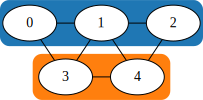
\includegraphics{figures/agg_example.pdf}
  \caption{Example graph.  The graph is partitioned into two aggregates.}
  \label{fig:example_graph}
\end{figure}

Denote $Agg$ the aggregation operator without smoothing, for example,
\begin{equation}
Agg =
\begin{bmatrix}
  1 & \\
  1 & \\
  1 & \\
  & 1 \\
  & 1
\end{bmatrix},
\end{equation}
would correspond to the above $5 \times 5$ system with two aggregates, the first containing nodes $0-2$ and the second containing nodes $3$ and $4$.  Let $\mat{A}$ be the system being solved and $\mat{P}$ the interpolation operator, i.e. that obtained by running some relaxation scheme on $Agg$.

One way to solve this is to first form $\mat{\hat{P}}$ as usual using the graphnet's node and edge convolutions.  This will give us a matrix that has the same sparsity pattern as $\mat{A}$.  Continuing the example from above, we may obtain some $\mat{\hat{P}}$ like
\begin{equation}
\mat{\hat{P}} =
\left[\begin{array}{@{}ccc|cc@{}}
  \sfrac{1}{2} & \sfrac{1}{3} & & & \\
  \sfrac{1}{2} & \sfrac{1}{3} & \sfrac{1}{3} & & \\
               & \sfrac{1}{3} & \sfrac{1}{3} & \sfrac{1}{3} &\\
               &              & \sfrac{1}{3} & \sfrac{1}{3} & \sfrac{1}{2} \\
  &              &              & \sfrac{1}{3} & \sfrac{1}{2}
\end{array}\right],
\end{equation}
with nodes to the left of the bar signifying those belonging to the first aggregate, and those to the right belonging to the second aggregate.

Then, we form $\hat{Agg}$, which is the $Agg$ operator from above except with its columns normalized in the $1$-norm.
\begin{equation}
\hat{Agg} =
\begin{bmatrix}
  \sfrac{1}{3} & \\
  \sfrac{1}{3} & \\
  \sfrac{1}{3} & \\
  & \sfrac{1}{2} \\
  & \sfrac{1}{2}
\end{bmatrix}.
\end{equation}
Now, we can ``collapse'' the columns of the nodes corresponding to each aggregate by averaging them together.  This can be written concretely as
\begin{equation}
\mat{P} = \mat{\hat{P}}\hat{Agg} = \begin{bmatrix}
  0.277 & \\
  0.333 & \\
  0.222 & 0.166 \\
  0.111 & 0.416 \\
  & 0.416 \\
\end{bmatrix},
\end{equation}
which gives a reasonable sparsity pattern for the interpolation, given $Agg$.  Note that if we view this as a graph, we get a 1-ring of edge connections around each aggregate.  A somewhat hand-wavy proof is given below.
\begin{proof}
  Assume that the entries of $\mat{\hat{P}}$ are strictly positive, which is reasonable because of the activation being used.  We can view the nonzero entries $\hat{p}_{ij}$ as edge connections from node $j$ to $i$.

  By averaging the columns $\vec{\hat{p}}_{i_1}, \vec{\hat{p}}_{i_2}, \ldots, \vec{\hat{p}}_{i_n}$ of an aggregate composed of nodes $i_1, i_2, \ldots, i_n$, we are obtaining the union of the neighborhood of each node in the aggregate, because all entries are positive.  Thus, an aggregate has connections to each node it is composed of, as well as the union of the neighbors of each node.
\end{proof}

\section{Full Algorithm}
Now that the average pooling technique has been introduced, the full algorithm for generating an interpolation operator $\mat{P}$ is defined below.
\begin{enumerate}
\item Given some sparse matrix $\mat{A}$, generate the graph $\mat{G}_{\mat{A}}$.
\item Create aggregates using some established clustering algorithm, such as Lloyd.  Store this as $Agg$ and form $\hat{Agg}$ by normalizing the columns.  Here, instead of normalizing the columns we are weighting them according to the output of a small 2-layer graphnet.
\item Create the binary inter-aggregate edge features $\theta_{ij}$ and append this to the edges of $\mat{G}_{\mat{A}}$.
\item Pass $\mat{G}_{\mat{A}}$ to the graphnet and obtain back $\mat{G}^\prime_{\mat{A}}$, which is a graph containing the same number of nodes and edges, but each having different weights.
\item Convert $\mat{G}^\prime_{\mat{A}}$ back into a matrix, we will denote this as $\mat{\hat{P}}$.
\item Finally, create $\mat{P}=\mat{\hat{P}}\hat{Agg}$.  This is our final interpolation operator.
\end{enumerate}

\section{Problem Description}
The problem being solved is a diffusion problem with Neumann boundary conditions.  The graphnet was trained on a randomly-generated training set of 3000 graphs, and separately evalutaed on a testing set of 200 graphs.

\section{Numerical Results}
The graphnet was allowed to train for approximately 9000 training iterations, and the performance relative to a Jacobi smoother is shown on the testing set (\ref{fig:loss_testing}) and training set (\ref{fig:loss_training}).  Something to note is that both training and testing losses seem to flatten after about 4000 iterations, then do not move at all.  I worry that our gradients may be vanishing and the optimizer cannot make any progress.

\begin{figure}[h]
  \includegraphics[width=\textwidth]{figures/graphnet_testing_loss.pdf}
  \caption{Loss of the testing dataset, showing the ML method and a baseline Jacobi smoother.  Note how the curve stagnates after 4000 or so iterations.}
  \label{fig:loss_testing}
\end{figure}

\begin{figure}[h]
  \includegraphics[width=\textwidth]{figures/graphnet_training_loss.pdf}
  \caption{Loss of the training dataset, showing the ML method and a baseline Jacobi smoother.  The curves are oscillatory due to the small batch sizes used.  One should interpret the relative performance as the distance between the two curves.}
  \label{fig:loss_training}
\end{figure}

\begin{figure}[h]
  \includegraphics[width=\textwidth]{figures/testing_conv_perf.pdf}
  \caption{Convergence factor of the ML method vs using the baseline Jacobi smoother on the testing set.  This is evaluated on an AMG solver for $\mat{Ax}=\vec{0}$ until $\normtwo{\vec{x}} \leq 10^{-10}$.}
  \label{fig:testing_perf}
\end{figure}

\begin{figure}[h]
  \includegraphics[width=\textwidth]{figures/training_conv_perf.pdf}
  \caption{Convergence factor of the ML method vs using the baseline Jacobi smoother on the training set.  This is evaluated on an AMG solver for $\mat{Ax}=\vec{0}$ until $\normtwo{\vec{x}} \leq 10^{-10}$.}
  \label{fig:testing_perf}
\end{figure}


\end{document}
